\documentclass[11pt,a4paper]{article}

\usepackage[margin=2.3cm]{geometry}
\usepackage[T1]{fontenc}
\usepackage{lmodern}
\usepackage{microtype}
\usepackage{graphicx}
\usepackage{booktabs}
\usepackage{tabularx}
\usepackage{float}
\usepackage{xcolor}
\usepackage{enumitem}
\usepackage[hidelinks]{hyperref}
\usepackage{caption}

\setlist{itemsep=2pt,topsep=4pt}
\setlength{\parskip}{4pt}
\captionsetup{font=small}


\title{\textbf{Guess the Rating}\\[4pt]
\large Estimating a chess player's blitz rating from one game}
\author{Raghava R (DA24B021)\\
DA3408 AI Operations, end-semester project\\
\small Code: \url{https://github.com/raghava137/guess-the-rating}}
\date{November 2026}

\begin{document}
\maketitle

\section{Introduction}

On Lichess every player has a rating, but it is built up over many games. In this project I
tried to go the other way: take a single blitz game and estimate the ratings of the two people
who played it. The app reads a Lichess game link or a pasted PGN, runs Stockfish over the moves,
looks at how each player used the clock, and returns an estimated rating with a range around it
and the three features that affected the estimate the most.

The model is only one part of the project. The rest is the system around it, as required for
this course: a DVC pipeline that can be re-run on any month of Lichess data, MLflow for
experiments and the model registry, a check before a new model is put into service, monitoring
with Prometheus and Grafana, alerts, and a web page to run the pipeline. All of it runs locally
in Docker Compose.

\section{Data}

The data comes from the Lichess open database, which publishes all rated games of each month as
one compressed PGN file (CC0 licence). I trained on July 2026 and used August 2026 to see how the
model does on a later month. These files are very large, so the ingest stage reads the file as
a stream and stops once it has collected enough games.

I only kept rated blitz games of standard chess. Lichess counts a game as blitz when the base time
plus 40 times the increment is between 180 and 479 seconds. Games with bot accounts and games that
ended in an unusual way were removed. Most players on Lichess are rated between 1200 and 1800, so
taking games at random would give very few weak or very strong players. To avoid this I split
ratings into ten bands (below 800, 800--999, \dots, 2400 and above) and kept up to 2,000 games per
band, using the average rating of the two players. A validation stage then parses each game
completely and removes very short games, games without clock times, games where a player
started with less time than the time control (berserk in arena tournaments) and duplicates.
Table~\ref{tab:data} shows the counts for July.

\begin{table}[H]
\centering
\caption{Data for the July 2026 run (\texttt{reports/ingest.json} and \texttt{reports/validation.json}).}
\label{tab:data}
\begin{tabular}{lr}
\toprule
Games read from the monthly file & 512,504 \\
\quad rejected: not blitz & 278,002 \\
\quad rejected: bot player & 2,689 \\
\quad rejected: unusual termination & 1,527 \\
\quad rejected: not rated & 1,042 \\
Games kept (2,000 in each of 10 bands) & 20,000 \\
\quad removed at validation: too short & 833 \\
\quad removed at validation: berserk / odd starting clock & 259 \\
\quad removed at validation: could not be read & 4 \\
Valid games & 18,917 \\
Rows for the model (one per player) & 37,834 \\
\bottomrule
\end{tabular}
\end{table}

For training and testing I split by player and not by game, using a hash of the username
(70\% train, 15\% validation, 15\% test). This way a player in the test set was never seen in
training, and because the hash does not change, the same player stays in the test set in the
next month as well.

\section{Features}

Each player in a game gets 17 features. Stockfish 15.1 analyses every position at depth 10, up to
the first 120 half-moves. From this I compute the average centipawn loss (ACPL) for the whole game
and separately for the opening, middlegame and endgame, the share of blunders, mistakes and
inaccuracies, and how often the player chose Stockfish's best move. From the clock times I compute
the share of the available time used, the average time per move, how much the move times vary,
how many moves were played with less than 10 seconds left, and whether the player lost on time.
The last few features are colour, game length, result and the opening family (ECO letter).

The ratings themselves, the rating difference and the player names are not used as inputs, and
one of the unit tests checks this. Stockfish is run with one thread and a fresh hash table for
every game. Without that, the same game could give slightly different features on different runs,
and the app uses the same feature code as training, so the features have to be reproducible.

\subsection*{A first look at the data}

Before training I looked at the features in the notebook \texttt{notebooks/eda.ipynb}, here on the
August data (18,825 games, 37,650 players). The opening ACPL has the strongest link with rating
(Spearman $-0.59$), followed by overall ACPL ($-0.49$), blunder rate ($-0.40$) and the share of
best moves ($+0.40$). Stronger players also move faster on average but vary their move times more.
Colour, result and losing on time are close to zero on their own, which is expected because both
players in a game have similar ratings. Table~\ref{tab:eda} shows that the bands are clearly ordered,
but neighbouring bands are only a few ACPL points apart, so one game cannot place a player exactly.

The endgame ACPL is missing for 58\% of players, because many games finish before an endgame, and
the middlegame ACPL for 0.7\%. LightGBM handles missing values itself, so I left them empty instead
of filling them in. Only 14 players had an ACPL above 300 and 286 used less than a tenth of their
clock. These are real games (mostly quick resignations), so I kept them.

\begin{table}[H]
\centering
\caption{Median values per rating band, August 2026.}
\label{tab:eda}
\begin{tabular}{lrrr}
\toprule
Band & ACPL & Blunder rate & Seconds per move \\
\midrule
below 800 & 88.8 & 0.08 & 6.14 \\
800--999 & 78.1 & 0.06 & 5.54 \\
1000--1199 & 70.8 & 0.05 & 5.03 \\
1200--1399 & 63.5 & 0.04 & 4.64 \\
1400--1599 & 58.6 & 0.04 & 4.38 \\
1600--1799 & 56.0 & 0.03 & 4.12 \\
1800--1999 & 51.3 & 0.03 & 3.94 \\
2000--2199 & 46.1 & 0.02 & 3.77 \\
2200--2399 & 40.3 & 0.02 & 3.72 \\
2400 and above & 36.2 & 0.00 & 3.41 \\
\bottomrule
\end{tabular}
\end{table}

\section{Model}

I used three LightGBM models trained on the same features. The middle one predicts the median
rating (L1 loss), and the other two are quantile models for the 10th and 90th percentile, so
together they give an estimate and a range that should contain the real rating about 80\% of the
time. The three ``reasons'' shown in the app are the feature contributions (SHAP values) of the
median model for that prediction. All three models are saved together as a single MLflow model.

As baselines I used the median rating of the training data (the same guess for everyone) and a
linear fit on ACPL alone.

\section{Results}

\begin{table}[H]
\centering
\caption{Results on test players. MAE and RMSE are in rating points. ``Within 200'' is the
fraction of estimates within 200 points of the real rating; coverage is the fraction of real
ratings inside the predicted range.}
\label{tab:results}
\begin{tabular}{lrr}
\toprule
 & July 2026 & August 2026 \\
 & (version 2) & (version 3) \\
\midrule
Test rows & 5,603 & 5,504 \\
MAE & \textbf{276.6} & \textbf{277.1} \\
RMSE & 352.7 & 355.7 \\
Within 200 points & 45.3\% & 45.2\% \\
Coverage of the range & 0.767 & 0.766 \\
Average width of the range & 851 & 852 \\
\midrule
Baseline: median rating & 483.2 & 484.8 \\
Baseline: linear fit on ACPL & 414.6 & 411.0 \\
\bottomrule
\end{tabular}
\end{table}

On July the model has an MAE of 276.6, against 483.2 for the median baseline and 414.6 for the
ACPL-only line, so the extra features do help. The range contains the real rating for 76.7\% of
test players, which is inside the 75--85\% I was aiming for.

To check the model on newer data, I ran the pipeline again on August. The July model (version 2)
had an MAE of 280.4 on the August test players, 3.8 points worse than on July and still well
below both baselines. The model trained on August (version 3) got 277.1, an improvement of 3.3
points. My promotion rule asks for at least 5 points, so version 3 was not put into service and
version 2 kept running. A difference of 3 points on one month is small enough to be noise, so I
was fine with this outcome.

\begin{figure}[H]
\centering
\begin{minipage}{0.48\textwidth}
  \centering
  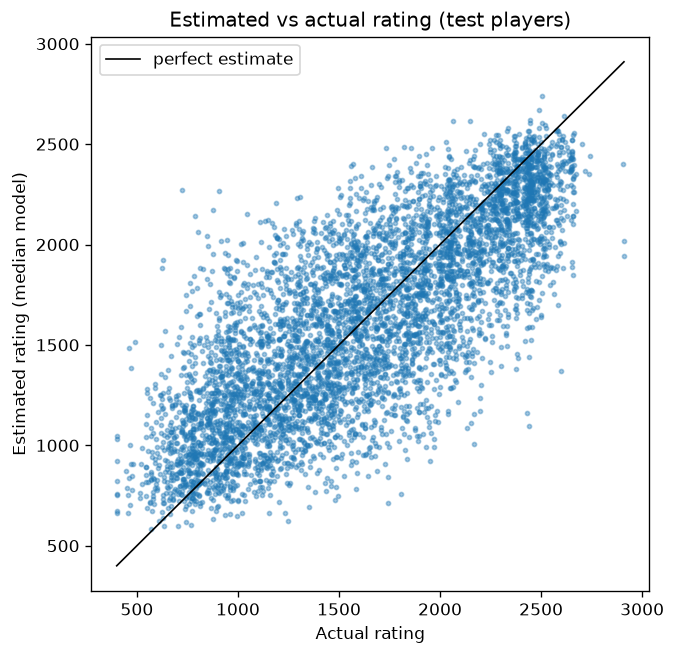
\includegraphics[width=\linewidth]{figures/pred_vs_actual.png}
  \caption{Estimated vs actual rating, July test players.}
  \label{fig:scatter}
\end{minipage}\hfill
\begin{minipage}{0.48\textwidth}
  \centering
  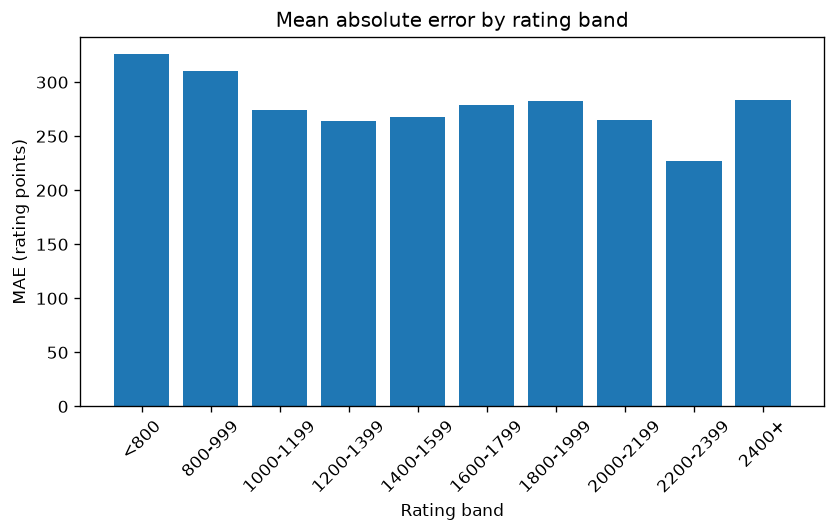
\includegraphics[width=\linewidth]{figures/band_mae.png}
  \caption{MAE for each rating band, July.}
  \label{fig:bands}
\end{minipage}
\end{figure}

In Figure~\ref{fig:scatter} the estimates are pulled towards the middle of the rating range.
Players rated around 500 are often estimated near 900, and players near 2500 are often estimated
around 2300. With only one game the model does not have much evidence for an extreme rating.
Figure~\ref{fig:bands} shows that the lowest bands have the largest error (326 below 800 and 310
for 800--999, compared to 227--284 for the other bands). Games between weak players vary a lot
from one game to the next, so a single game is less informative.

\begin{figure}[H]
\centering
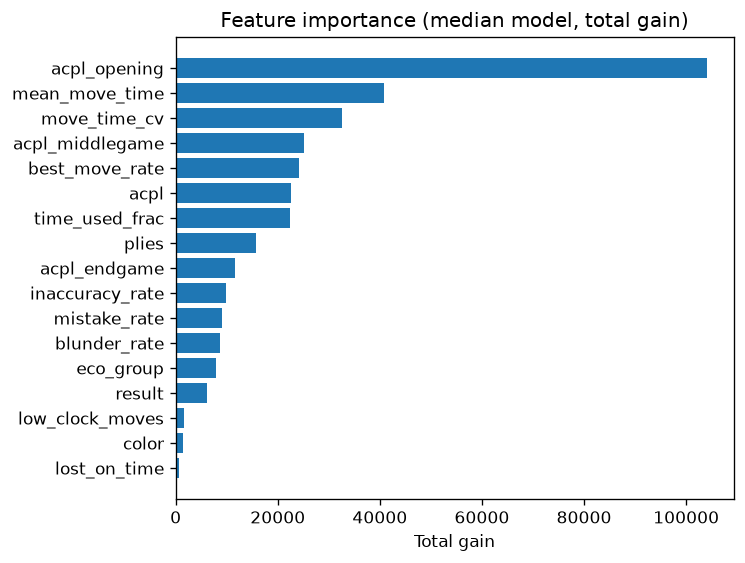
\includegraphics[width=0.62\textwidth]{figures/feature_importance.png}
\caption{Feature importance of the median model (total gain).}
\label{fig:importance}
\end{figure}

The most important feature by far is the ACPL in the opening (Figure~\ref{fig:importance}),
more than the ACPL over the whole game. A possible reason is that stronger players know their
openings well and lose very little in the first ten moves, while later in the game the ACPL also
depends on how the position went. The next most important features are the average time per move
and how much the move times vary, so the way a player uses the clock in blitz tells the model
quite a lot.

\section{System}

\begin{figure}[H]
\centering
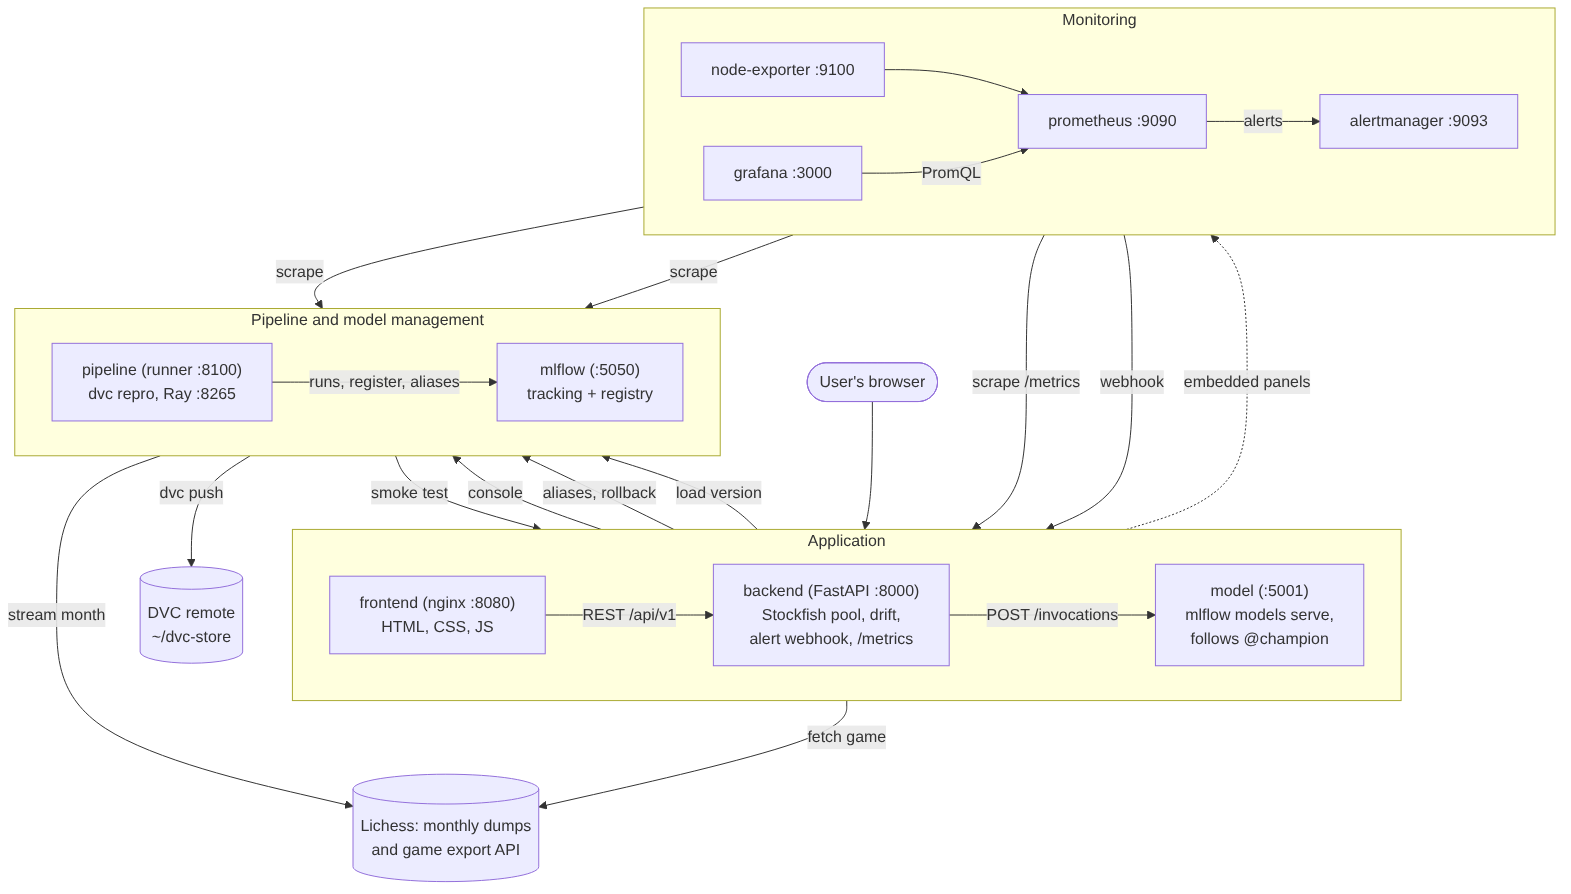
\includegraphics[width=\textwidth]{figures/architecture.png}
\caption{Architecture of the app (nine Docker Compose services).}
\label{fig:arch}
\end{figure}

Figure~\ref{fig:arch} shows the services. The web page is served by nginx and only talks to the
FastAPI backend through a REST API. The backend parses the game, computes the features with
Stockfish using the same code as the pipeline, and sends them to the MLflow model server. The
model server always serves the model version that has the \texttt{@champion} alias in the MLflow
registry and reloads by itself when the alias changes. Prometheus, Alertmanager, Grafana and
node-exporter are used for monitoring.

\subsection{Pipeline}

The pipeline has six DVC stages: ingest, validate, featurize, train, evaluate and promote. The
settings are all in \texttt{params.yaml}, and \texttt{dvc repro} only runs stages whose code,
data or settings changed. The data and models are DVC outputs and are pushed to a local DVC
remote, and I commit \texttt{dvc.lock} after each run. The training stage is run as an MLflow
project and logs the month, the number of games, the Stockfish version and depth, the Git commit
and a hash of the feature file, together with metrics, plots and the drift reference. With the
commit and the MLflow run ID any model can be traced back to the code and data that produced it.

The validate stage splits the games into chunks and processes them as Ray tasks. Featurize uses a
pool of Ray actors, where each actor has its own Stockfish process. Table~\ref{tab:speed} shows
the times for the July run.

\begin{table}[H]
\centering
\caption{Stage times for the July run on my Mac (Docker with 12 CPUs and 13.9 GB). Total 86 minutes.}
\label{tab:speed}
\begin{tabular}{lrrr}
\toprule
Stage & Time & Workers & Throughput \\
\midrule
ingest & 3 min & 1 & 3,374 games read / s \\
validate & 27 s & 8 Ray tasks & 764 games / s \\
featurize & 83 min & 10 Ray actors & 3.82 games / s \\
train & 11 s & & \\
evaluate & 4 s & & \\
promote (with smoke test) & 18 s & & \\
\bottomrule
\end{tabular}
\end{table}

Almost all of the time is spent in featurize, since every position of 18,917 games goes through
Stockfish. This is the stage where using Ray makes the biggest difference, because the work is
split over ten processes.

\subsection{Promotion and rollback}

After evaluation, the new model only replaces the current one if three conditions hold: its range
contains between 75\% and 85\% of the real test ratings, it is better than the median baseline,
and its MAE is at least 5 points lower than the current model's MAE on the same test players. If
it passes, \texttt{@previous} is set to the old version and \texttt{@champion} to the new one, the
model server loads it, and a smoke test sends three real games through the backend. If the smoke
test fails, the aliases are changed back automatically. There is also a rollback button on the
pipeline page.

\begin{figure}[H]
\centering
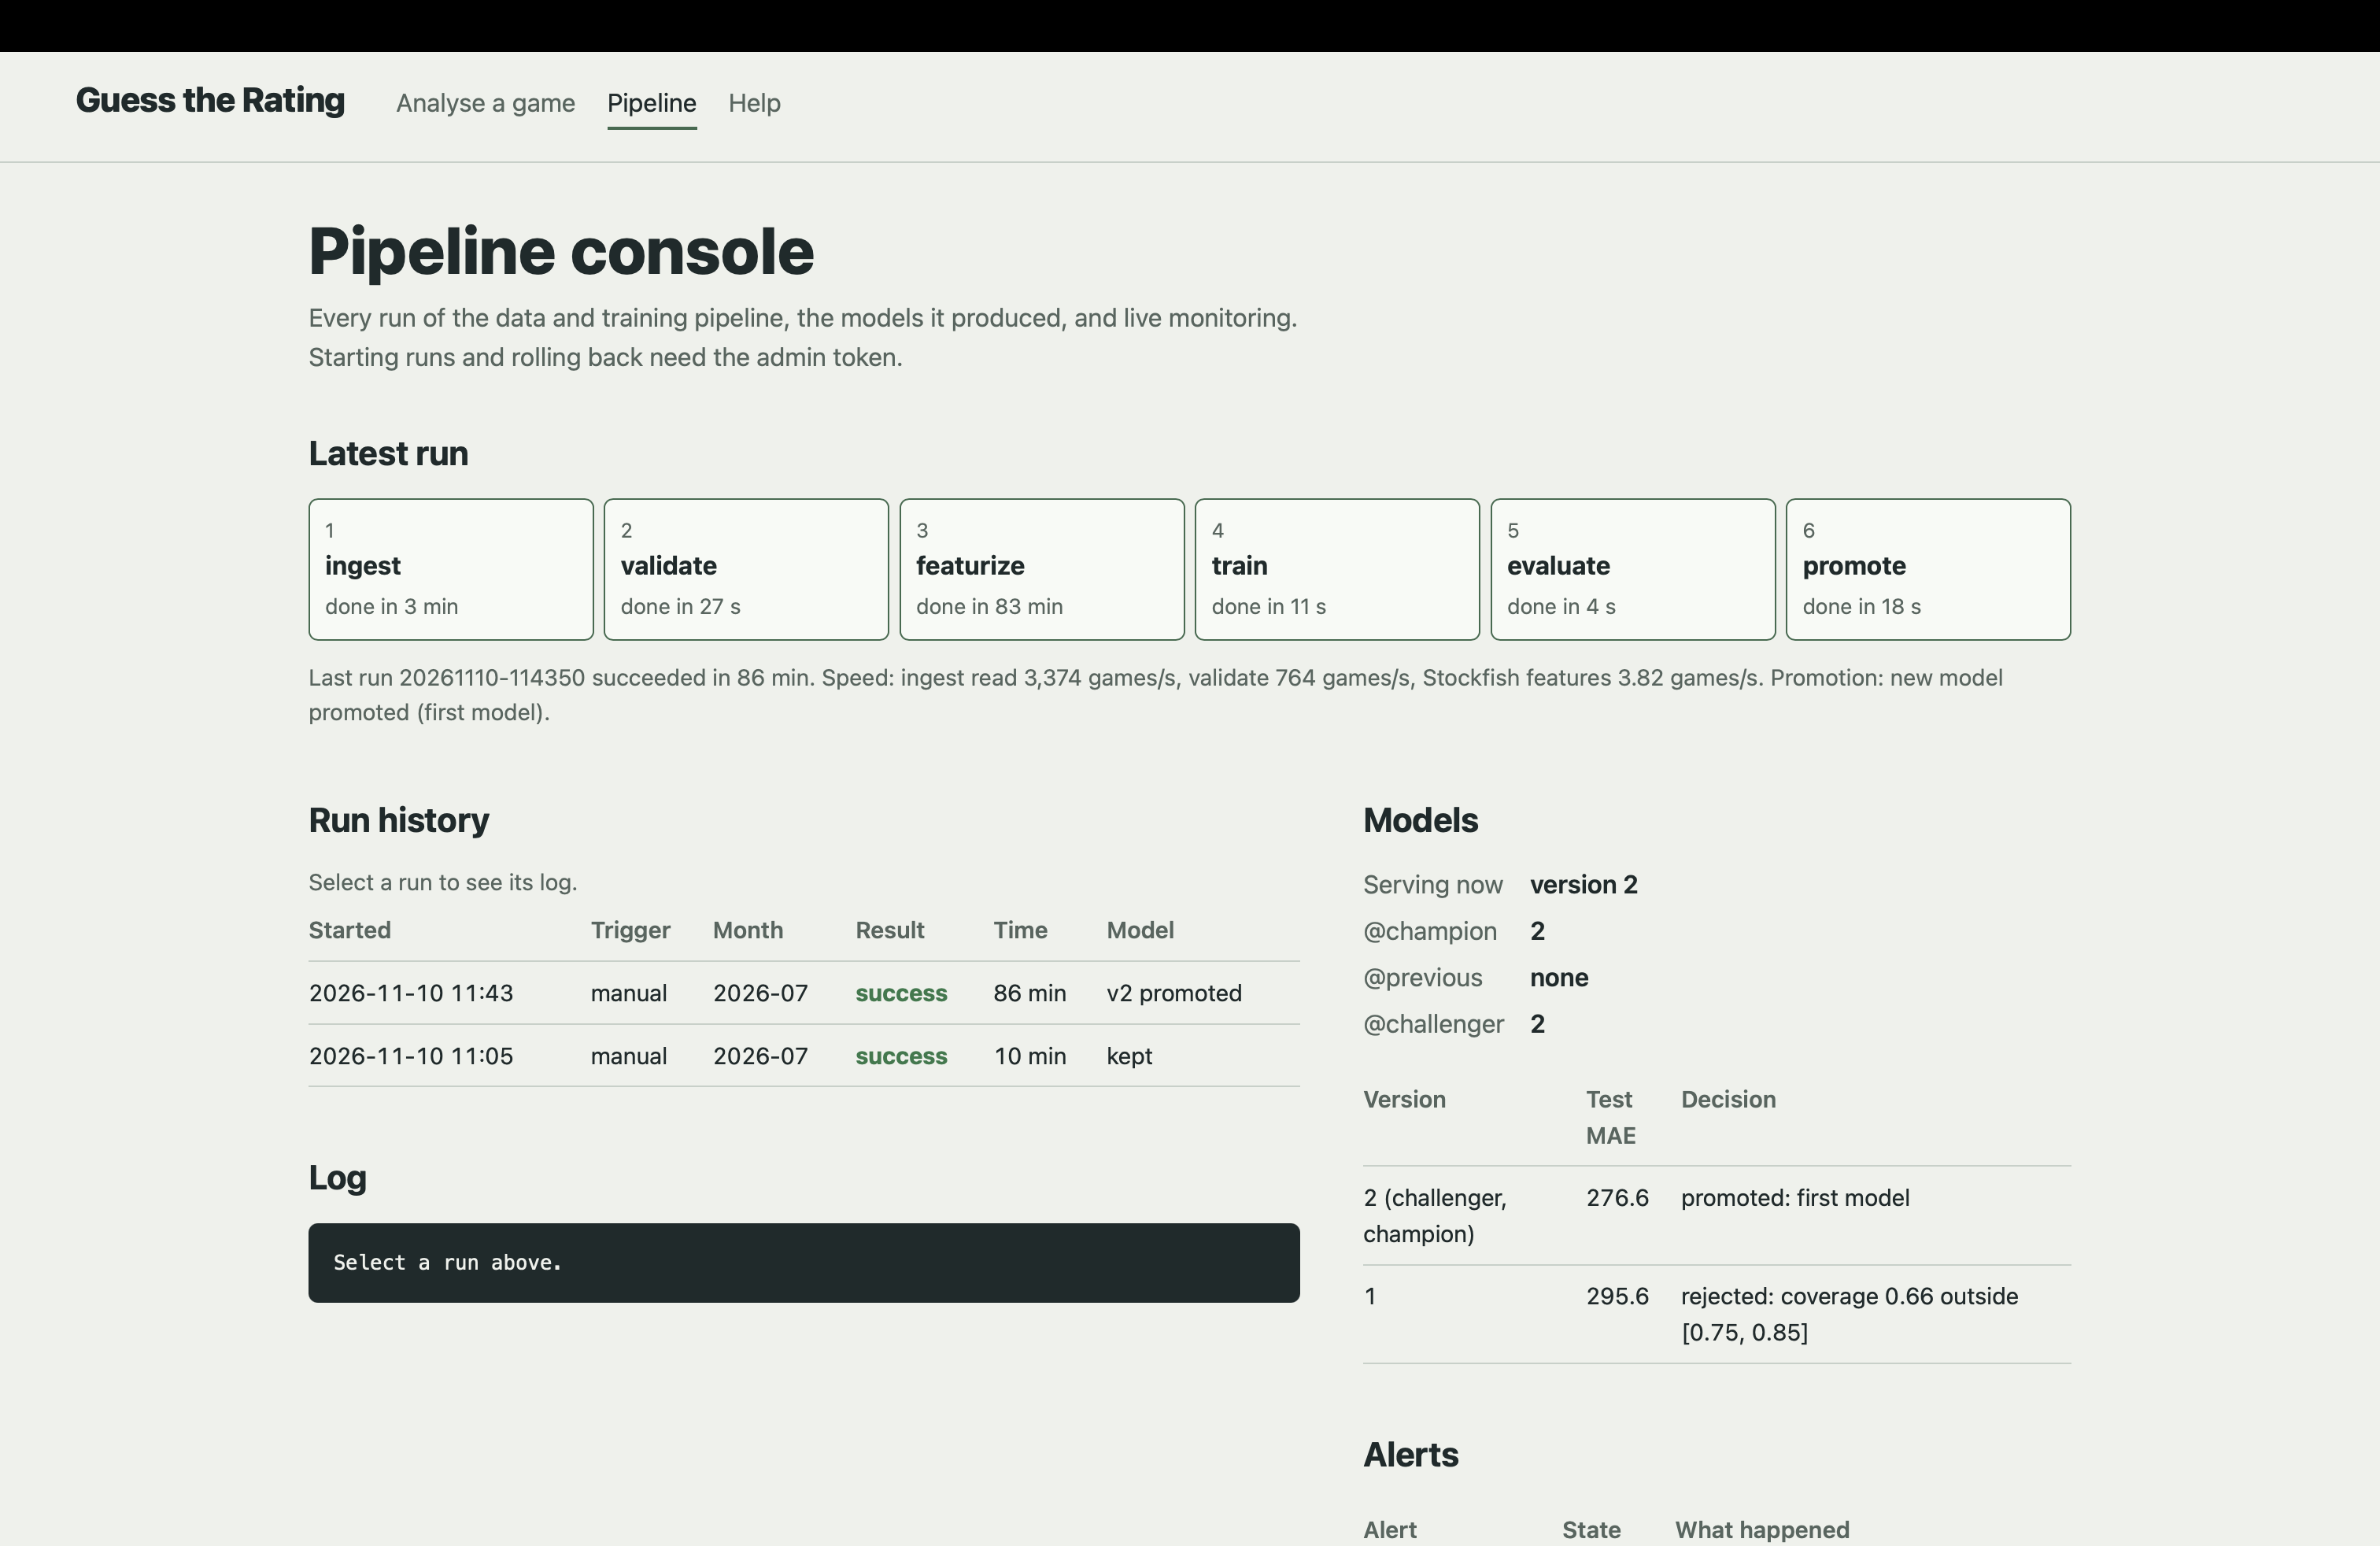
\includegraphics[width=\textwidth]{figures/pipeline_console.png}
\caption{Pipeline page after the July run. Version 1 came from a small trial run with 200 games
per band; its range covered only 66\% of test players, so it was rejected. Version 2 was promoted.}
\label{fig:console}
\end{figure}

\subsection{Monitoring}

Prometheus scrapes the backend, the pipeline runner, MLflow, Alertmanager, Grafana, node-exporter
and itself, and the backend checks the model server and the frontend every 15 seconds. The
backend reports request counts, latency, Stockfish time, rejected games by reason, and the error
on live games whose real rating is known (Lichess games include it). For data drift it computes
the population stability index (PSI) of ACPL, time per move and game length for the last 200
players, compared with the training data.

There are seven alert rules: a service or scrape target going down, too many server errors, slow
predictions, drift, a high live error, and a failed pipeline run. Alertmanager sends alerts to
the backend, which lists them on the pipeline page. If \texttt{AUTO\_RETRAIN} is set to true, a
drift or live-error alert starts a pipeline run on the next month, at most once a day.

Starting a run or rolling back needs an admin token stored in \texttt{.env}, which is not
committed. The prediction log is encrypted with Fernet and does not store player names.

\section{Testing}

There are 70 unit and API tests, and all of them pass. A Git pre-push hook runs flake8, the tests
and \texttt{dvc status} inside the Docker image before every push. All seven Prometheus targets
were up.

I sent 100 normal games and 120 long games through the running app and all of them were answered
with HTTP 200. Bad inputs, such as plain text or a link to another website, got an HTTP 422
with a plain message like ``That does not look like a Lichess game link''. The long games (all over 100 half-moves) changed the distribution of game length compared to
training, and the PSI for game length went up to 6.25, far above the 0.2 limit. FeatureDrift went
to pending and then fired after 10 minutes (Figure~\ref{fig:drift}). Automatic retraining was
switched off, so it only showed up as an alert. The ComponentDown alert fired while there was no
model to serve, before the first promotion, and resolved after it.

\begin{figure}[H]
\centering
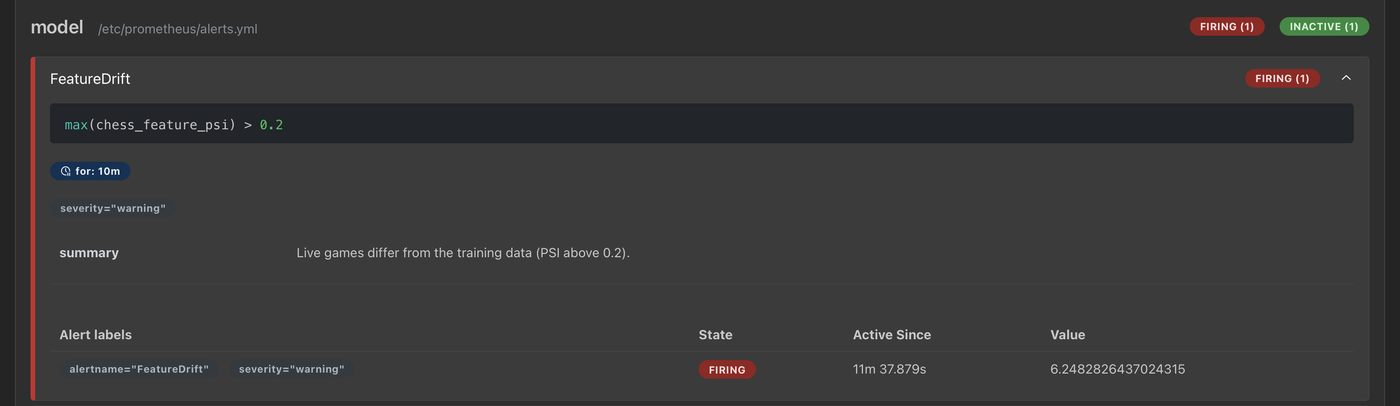
\includegraphics[width=\textwidth]{figures/feature-drift-firing.png}
\caption{FeatureDrift firing in Prometheus after the drift test.}
\label{fig:drift}
\end{figure}

 Table~\ref{tab:load} shows the load test.

\begin{table}[H]
\centering
\caption{Load test with \texttt{scripts/load\_test.py}.}
\label{tab:load}
\begin{tabular}{rrrrrl}
\toprule
Clients & Requests & Throughput & p50 & p95 & Status \\
\midrule
1 & 10 & 0.56 req/s & 1.60 s & 2.90 s & all 200 \\
4 & 40 & 1.08 req/s & 3.70 s & 5.24 s & all 200 \\
\bottomrule
\end{tabular}
\end{table}

With one client the 95th percentile latency is 2.9 s, below my 5 s target. With four clients it
goes up to 5.2 s. The backend has two Stockfish engines, so only two games are analysed at the
same time and the other requests wait. Adding engines (and CPU cores) would increase the
throughput.

\begin{table}[H]
\centering
\caption{Acceptance criteria from the test plan.}
\begin{tabularx}{\textwidth}{lXl}
\toprule
 & Criterion & Status \\
\midrule
AC1 & MAE beats both baselines on next month's test players & Met (280.4 vs 484.8 / 411.0) \\
AC2 & Coverage between 75\% and 85\% & Met (0.767 and 0.766) \\
AC3 & p95 under 5 s for one user & Met (2.90 s) \\
AC4 & Tests pass, flake8 clean & Met (70/70) \\
AC5 & Readable 4xx for invalid input, no 500s & Met (HTTP 422 with a plain message; no 500s) \\
AC6 & Whole stack starts with one \texttt{docker compose up} & Met (9 services) \\
AC7 & A fresh clone reproduces the metrics & Not repeated on my machine \\
AC8 & Every component up; each alert fires in a forced test & Partly (all up; 2 of 7 alerts forced) \\
AC9 & A broken model is rolled back automatically & Not repeated on my machine \\
\bottomrule
\end{tabularx}
\end{table}

\section{Limitations and future work}

One game is a small sample, and the predicted range is about 850 points wide on average. Using
several games of the same player would make it much narrower. The estimates are also pulled
towards the middle, so very weak and very strong players are not estimated well. The model only
knows Lichess blitz, and other sites or time controls have different rating scales.

On the system side, a promotion restarts the single model server, so predictions fail for a few
seconds while the new version loads. Running two model servers and switching between them would
avoid this. Stockfish at depth 10 is weaker than a full analysis; since training and the app use
the same depth this is consistent, but a deeper analysis might help for the strongest players.

\appendix
\section{Running the project}

\begin{verbatim}
cp .env.example .env          # add ADMIN_TOKEN and FERNET_KEY
mkdir -p ~/dvc-store
docker compose up -d --build
# then open http://localhost:8080/pipeline.html and start a run
\end{verbatim}
The README in the repository has the full setup and commands, and the \texttt{docs/} folder has
the architecture, high- and low-level design, test plan, test report and user manual.

\end{document}
